\chapter{Synchronization Tools}


\section{Critical section and race condition}
For now we know: to create tasks, the tasks have a own life, scheduling algorithms. But how we manage it?

\paragraph{Problem:} in a dual core processor each process has own life, if in the same time two process call the fork() call, the sub-processes have the same PID! This may happen because in the dual-core processor the tasks are execute in parallel. 

\paragraph{}
This problem also happen even if we have a single-core CPU, because if the OS has the preemption mechanism in each time the function fork() can be kicked out of the CPU before increase the PID number, the another tasks call the same function and after that we have the same problem saw before: two tasks with same PID.

\paragraph{}
This is called \textbf{race condition}, and implies the inconsistency of the data read. We want to maintaining this consistency of data.

\paragraph{NOTA:} the race condition and the inconsistency of the data happen \textbf{only} if the variable is in the read/write mode, this not happen if the variable is only in read mode!


\begin{figure}[htbp]
    \centering
    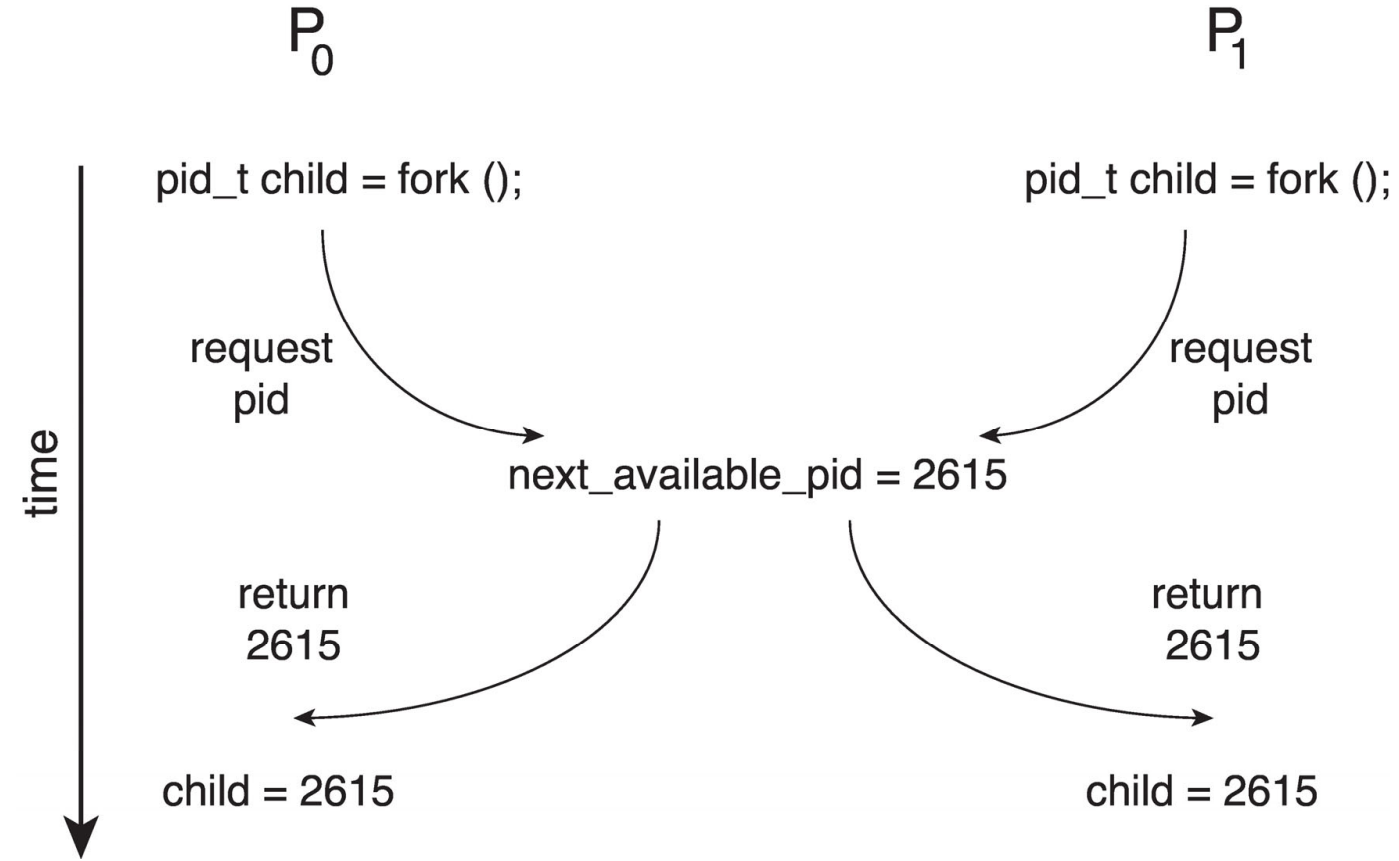
\includegraphics[width=0.65\linewidth]{img/race_cond.png}
    \caption{Race condition on kernel variable next\_available\_pid}    
\end{figure}


\newpage
\subsection{Critical section}
Consider system of n processes, each process has critical section segment of code: process may be changin common variables, updating tables, etc.

When one process in critical section, no other may be in its critical section, \textbf{Critical section problem} is to design protocol to solve this.

Each process must:

\begin{itemize}
    \item ask permission to enter critical section in entry section,
    \item may follow critical section with exit section,
    \item then remainder section
\end{itemize}

\begin{codeInC}
while( true ){
    ...
    
    //entry into critical section
        critical section
    //exit critical section
    
    ...
}
\end{codeInC}


\subsection{Critical section problem}
Requirements for solution to critical-section problem:

\begin{itemize}
    \item \textbf{Mutual Exclusion} - If process Pi is executing in its critical section, then no other processes can be executing in their critical sections; no more one in the same critical section;
    \item \textbf{Progress} - If no process is executing in its critical section and there exist some processes that wish to enter their critical section, then the selection of the process that will enter the critical section next cannot be postponed indefinitely; if no one tasks are into the critical section other process may access into it;
    \item \textbf{Bounded Waiting} - A bound must exist on the number of times that other processes are allowed to enter their critical sections after a process has made a request to enter its critical section and before that request is granted; if a tasks want to enter into the critical section must waiting to have the access.
\end{itemize}

If your system has a \textbf{single core} CPU and is \textbf{nonpreemtive} OS, you never have this problem, but the question is: who in 2024 does not have a multi-core CPU inside a PC? None.
\newpage
\section{Software solutions 1}
Assume that the \textbf{load} and \textbf{store} machine-language instructions are atomic; that is, cannot be interrupted. 

Two processes share one variable called: int turn, this variable indicates who can access the critical section. Initially, the value of turn is set to i.

\begin{codeInC}
while (true){
    while (turn = = i);
    /* critical section */
    turn = i;
    /* remainder section */
}
\end{codeInC}


\begin{codeInC}
while (true){
    while (turn = = j);
    /* critical section */
    turn = j;
    /* remainder section */
}
\end{codeInC}

\paragraph{Correctness of this Software Solution:} 

\begin{itemize}
    \item \textbf{Mutual exclusion} is preserved, since Pi enters critical section only if turn == i;
    \item \textbf{Progress requirements} is not respected. The other task can not access into its critical section;
    \item \textbf{Bounded-waiting}, also, is not respected. Process J may be waiting for the critical section endlessly.
\end{itemize}


\subsection{Peterson’s Solution}

Same as before: two process, load and store machine-language instructions are atomic.

The change is: two processes share two variables: int turn and boolean flag[2]. The first indicates which processes enters the critical section, and the flag array is used to indicate if a process is ready to enter the critical section, flag[i] = true -> the process Pi is ready.

\paragraph{Peterson’s Algorithm for Process Pi}


\begin{codeInC}
while (true){
    flag[i] = true;
    turn = j;
    while (flag[j] && turn = = j);
    
    /* critical section */
    
    flag[i] = false;
    
    /* remainder section */
}
\end{codeInC}

\newpage
\paragraph{Correctness of Peterson’s Solution:} 

\begin{itemize}
    \item \textbf{Mutual exclusion} is preserved, since Pi enters critical section only if turn == i, either flag[j] = false or turn = i;
    \item \textbf{Progress requirements} is satisfied.
    \item \textbf{Bounded-waiting}, requirement is met. If it is the turn of the other, but the other is not willing to enter the critical
section, the first process will enter (even if not its turn technically).
\end{itemize}

Although useful for demonstrating an algorithm, Peterson’s
Solution is not guaranteed to work on modern architectures. To improve performance, processors and/or compilers may
reorder operations that have no dependencies.

For single-threaded this is ok as the result will always be the
same. 
For multithreaded the reordering may produce inconsistent or
unexpected results! Ideally, you want a single instruction for entry/exit section.

\subsection{Reordering}

The compiler transform the high programme language into binary code, but for optimization it happen that some operation are physically distant, and the preemption could cause some error.

\subsection{Peterson vs Multi-Threading}
The effects of instruction reordering in Peterson’s Solution

\begin{figure}[htbp]
    \centering
    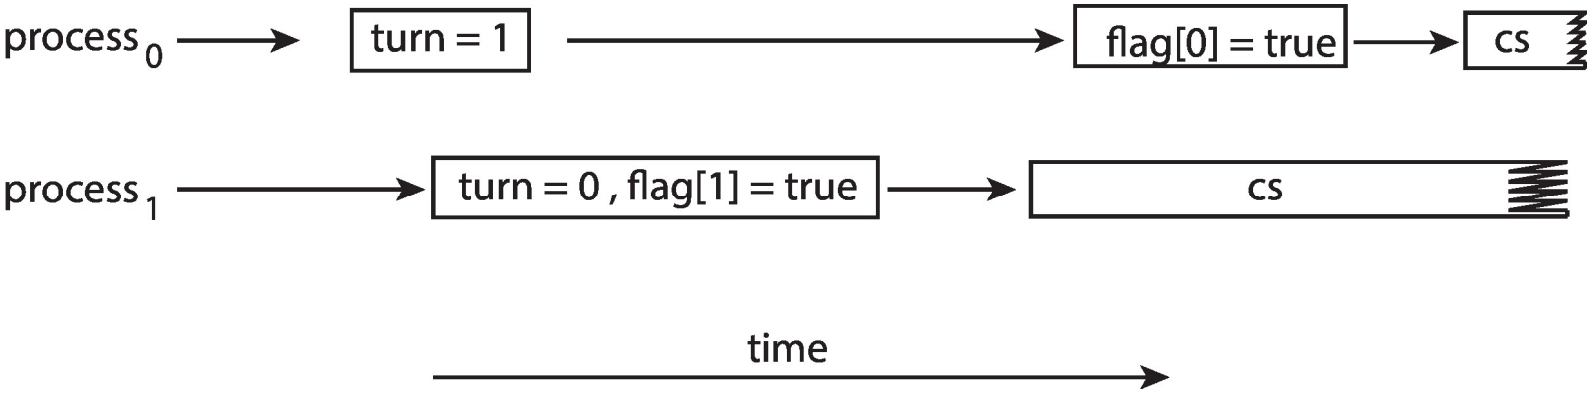
\includegraphics[width=0.65\linewidth]{peterson.png}    
    
\end{figure}

This allows both processes to be in their critical section at the same
time, to ensure that Peterson’s solution will work correctly on modern
computer architecture we must use a \textbf{Memory Barrier}.
\newpage
\section{Memory Barrier}

Memory models may be either:

\begin{itemize}
    \item \textbf{Strongly ordered} – where a memory modification of one processor is immediately visible to all other processors.
    \item \textbf{Weakly ordered} – where a memory modification of one processor may not be immediately visible to all other processors
\end{itemize}

A memory barrier is an instruction that forces any change in memory to be propagated (made visible) to all other processors.

\paragraph{}
I need some barrier line that tells to compiler that it can reorder instruction before and after the barrier. In this way the consisntency of the data are ok.

\paragraph{Example:} boolean flag = false; int x = 0;
\begin{codeInC}
//thread one
while (!flag)

memory_barrier();
print x;
\end{codeInC}
\begin{codeInC}
//thread two
while (!flag)

memory_barrier();
print x;
\end{codeInC}

For Thread 1 we are guaranteed that that the value of flag
is loaded before the value of x.

For Thread 2 we ensure that the assignment to x occurs
before the assignment flag.

\paragraph{}
If we do not write \verb|memory_barrier();| the programm print the value of 0, before the value x is set bt thread 2.

\newpage
\section{Hardware instructions}

How to implement all of this in the language programm?

\paragraph{}
Many systems provide hardware support for implementing the critical section code.
We will look at three forms of hardware support:
\begin{itemize}
    \item Hardware instructions
    \item Atomic variables
\end{itemize}

\subsection{Hardware Instructions}
Special hardware instructions that allow us to either
test-and-modify the content of a word, or to swap the
contents of two words atomically: 

\begin{itemize}
    \item[] Test-and-Set instruction
    \item[] Compare-and-Swap instruction
\end{itemize}


\subsubsection{test\_and\_set instruction}

\begin{codeInC}
boolean test_and_set (boolean *target){
    boolean rv = *target;
    *target = true;
    return rv:
}
\end{codeInC}

Properties:

\begin{itemize}
    \item Executed atomically
    \item Returns the original value of passed parameter
    \item Set the new value of passed parameter to true
    \item No changes if target is already true
\end{itemize}

Shared boolean variable lock, initialized to false:

\begin{codeInC}
do {
    while (test_and_set(&lock)); /* do nothing */
    /* critical section */
    lock = false;
    /* remainder section */
} while (true);

\end{codeInC}

After the first process, any process can go in. There is no
queue maintained, so any new process that finds the lock to
be false again can enter. So bounded waiting is not
ensured.

\paragraph{}
The \verb|lock| is:

\begin{itemize}
    \item \textbf{false} when the critical section is empty (not busy);
    \item \textbf{true} when the critical section is full (busy);
\end{itemize}

The \verb|Test_and_set| function guarantee the mutual exclusion and the progress, but does not guarantee bounded waiting!


\subsubsection{compare\_and\_swap instruction}
This hardware instruction first reed the lock value, then set a specific value.

\begin{codeInC}
int compare_and_swap(int *value, int expected, int new_value) {
    int temp = *value;
    if (*value == expected)
    *value = new_value;
    return temp;
} 

\end{codeInC}

Properties:

\begin{itemize}
    \item Executed atomically
    \item Returns the original value of passed parameter value
    \item Set the variable value the value of the passed parameter new\_value but only if *value == expected is true.
    \item That is, the swap takes place only under this condition
\end{itemize}

Solution using \verb|Test_and_set| and shared integer lock initialized to 0.
\begin{codeInC}
while (true){
    while (compare_and_swap(\&lock, 0, 1) != 0); /* do nothing */
    /* critical section */
    lock = 0;
    /* remainder section */
}

\end{codeInC}

But this solution can resolve the previous problem?

\begin{itemize}
\centering
    \item[] Mutual exclusion: yes
    \item[] Progress: yes
    \item[] Bounded Waiting: no
\end{itemize}

To solve this we can rewrite the code as following:


\begin{codeInC}
while (true) {
    waiting[i] = true;
    key = 1;
    while (waiting[i] && key == 1)
        key = compare_and_swap(&lock,0,1);
    waiting[i] = false;
    
    /* critical section */
    j = (i + 1) \% n;
    while ((j != i) && !waiting[j])
        j = (j + 1) \% n;
        
    if (j == i)
        lock = 0;
    else
        waiting[j] = false;
    /* remainder section */
}

\end{codeInC}

Here is where the bounded
waiting is guaranteed
Scans from i+1 to n to 0 to
i-1 for a process waiting in
the CS.

\paragraph{}
In this way we are create a looping queue, so if a process exit to the critical section, it passes the control to the next process and not to the tasks that got the lock before anyone. This guarantees that any process, who willing into the critical section, sooner or later will enter into it.


In this way the \textbf{bounded waiting} is guarantee.

\section{Atomic Variables}
Typically, instructions such as compare-and-swap are used as building blocks for other synchronization tools. Using atomic variables provides \textbf{atomic} updates on a basic data type such as integer and booleans.


\paragraph{Example: } Let \textbf{sequence} be an atomic variable, Let \textbf{increment()} be operation on the atomic variable
sequence. The command \verb|increment(&sequence);| ensures sequence is incremented without interruption:

\begin{codeInC}
void increment(atomic_int *v){
    int temp;
    do {
        temp = *v;
    }while (temp != (compare_and_swap(v,temp,temp+1));
}

\end{codeInC}

\section{Mutex Locks}

Previous solutions are complicated and generally inaccessible to
application programmers, OS designers build software tools to solve critical section problem, the simplest is \textbf{mutex lock} a boolean variable indicating if lock is available or not. It protect the critical section by:

\begin{itemize}
    \item First \textbf{acquire()} a lock;
    \item Then \textbf{release()} the lock.
\end{itemize}

Usually implemented via hardware atomic instructions such as
compare-and-swap. But this solution requires \textbf{busy waiting}, this lock therefore called a \textbf{spinlock}.


\begin{codeInC}
while (true) {
    acquire lock
        critical section
    release lock
    
    remainder section
} 

\end{codeInC}


If not free, you will be blocked on “acquire” until it releases. This is the “busy wait”, you cant do anything else while you wait, so you are subtract useful work to the CPU.

\newpage
\section{Semaphore}

I will not subtract useful work to the CPU, so we want someone who notify to the task when a specific resource, in this case the critical section, i free to entry. 

Semaphore is a \textbf{synchronization tool}, and not only a way to enter into a critical section, that provides more sophisticated ways, than mutex locks, for processes to synchronize their activity.  With semaphores we can solve various synchronization problems.

\paragraph{}
Semaphores can only be accessed via two atomic operations:

\begin{itemize}
    \item wait()
    \item signal()
\end{itemize}

\subsection{Definition of the wait operation}

\begin{codeInC}
wait(S) {
    while (S <= 0); // busy wait
    S--;
}

\end{codeInC}

\subsection{Definition of the signal operation}

\begin{codeInC}
signal(S) {
    S++;
} 
\end{codeInC}

The are two different type of semaphores:

\begin{itemize}
    \item \textbf{Counting semaphore} – integer value can range over an unrestricted domain
    \item \textbf{Binary semaphore} – integer value can range only between 0 and 1, this is equivalent to mutex lock
\end{itemize}

It is possible to implement a counting semaphores as a binary semaphores.

\paragraph{Semaphores usage example:} Solution to CS problem creating a semaphores "mutex" initialized to 1

\begin{codeInC}
wait(mutex);
    CS
signal(mutex);
\end{codeInC}

Consider P1 and P2 that with two statements S1 and S2 and
the requirement that S1 to happen before S2. Create a semaphore “synch” initialized to 0.

\begin{codeInC}
P1:
    S1;
    signal(synch);
P2:
    wait(synch);
    S2;
\end{codeInC}

All works good but there are still busy waiting, \textbf{spinlock}! We can do better!

\newpage
\subsection{Semaphore Implementation with no Busy waiting}
With each semaphore there is an associated waiting queue, a list of a processes willing to enter into the critical section.

Each entry in a waiting queue has two data items:

\begin{itemize}
    \item Value (of type integer);
    \item Pointer to next record in the list, single(ahead)-pointer linked list.
\end{itemize}

Also there are two operations:

\begin{itemize}
    \item \textbf{block} – place the process invoking the operation on the appropriate waiting queue
    \item \textbf{wakeup} – remove one of processes in the waiting queue and place it in the ready queue
\end{itemize}


\begin{codeInC}
wait(semaphore *S) {
    S->value--;
    if (S->value < 0) {
        add this process to S->list;
        block();
    }
}
\end{codeInC}


\begin{codeInC}
signal(semaphore *S) {
    S->value++;
    if (S->value <= 0) {
        remove a process P from S->list;
        wakeup(P);
    }
}    
\end{codeInC}

The struct of semaphores with waiting queue is:

\begin{codeInC}
typedef struct {
    int value;
    struct process *list;
} semaphore; 
\end{codeInC}

\subsection{Problems with semaphores}

If a programmer do not take care when use signal and wait, the semaphores work in a bad way! Some example could be:

\begin{itemize}
    \item[] Omitting the wait: you forget that you are using the critical section;
    \item[] Omitting the signal: you exit the critical section without notify that.
\end{itemize}

\newpage
\section{Monitors}
Another high-level abstraction tools used for synchronization is called \textbf{monitors}. 

Pseudocode syntax of a monitor:

\begin{codeInC}
monitor monitor-name{
    // shared variable declarations
    procedure P1 (...) { ... }
    procedure P2 (...) { ... }
    procedure Pn (...) { ... }
    initialization code (...) { ... }
}
\end{codeInC}

You can see it as a service that you can call:

\begin{itemize}
    \item It offers some functions;
    \item You don’t worry about critical sections, parallelism, whatsoever;
    \item The monitor itself is managing them (mutual exclusion, progress);
    \item It will answer eventually (bounded waiting).
\end{itemize}


\begin{figure}[htbp]
    \centering
    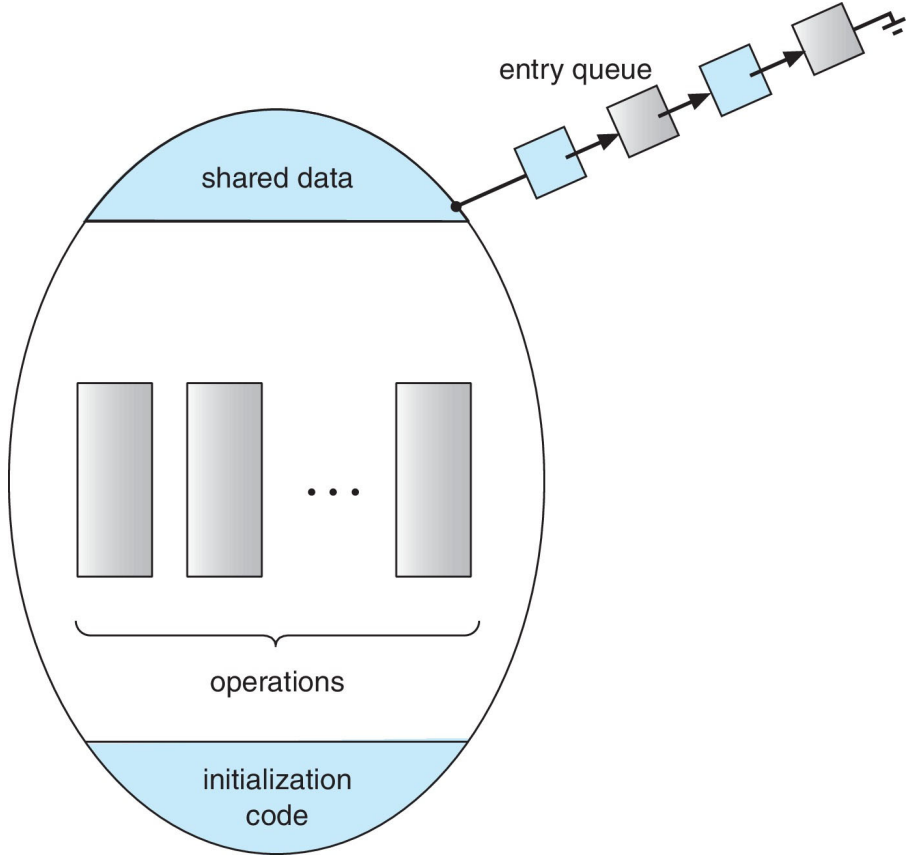
\includegraphics[width=0.45\linewidth]{img/monitors.png}
    \caption{Schematic view of a Monitor}
\end{figure}


\subsection{Monitor Implementation Using Semaphores}

Variables: semaphore mutex, mutex = 1.
\paragraph{}
Each procedure P is replaced by :

\begin{codeInC}
wait(mutex);
    ...
    body of P;
    ...
signal(mutex);
\end{codeInC}

\textbf{Mutual exclusion} within a monitor is ensured.

However, what if procedures need to interact in the critical section?


Maybe a procedure can be ran until a given point but then needs some
action by another process?

\subsection{Condition Variables}
Monitors allow for the creation of condition variables: \textbf{condition x, y;}

Two operations are allowed on a condition variable:

\begin{itemize}
    \item \textbf{x.wait()} – a process that invokes the operation is suspended until x.signal();
    \item \textbf{x.signal()} – resumes one of processes (if any) that invoked x.wait(), if not any then it has no effect on the variable
\end{itemize}

\begin{figure}[htbp]
    \centering
    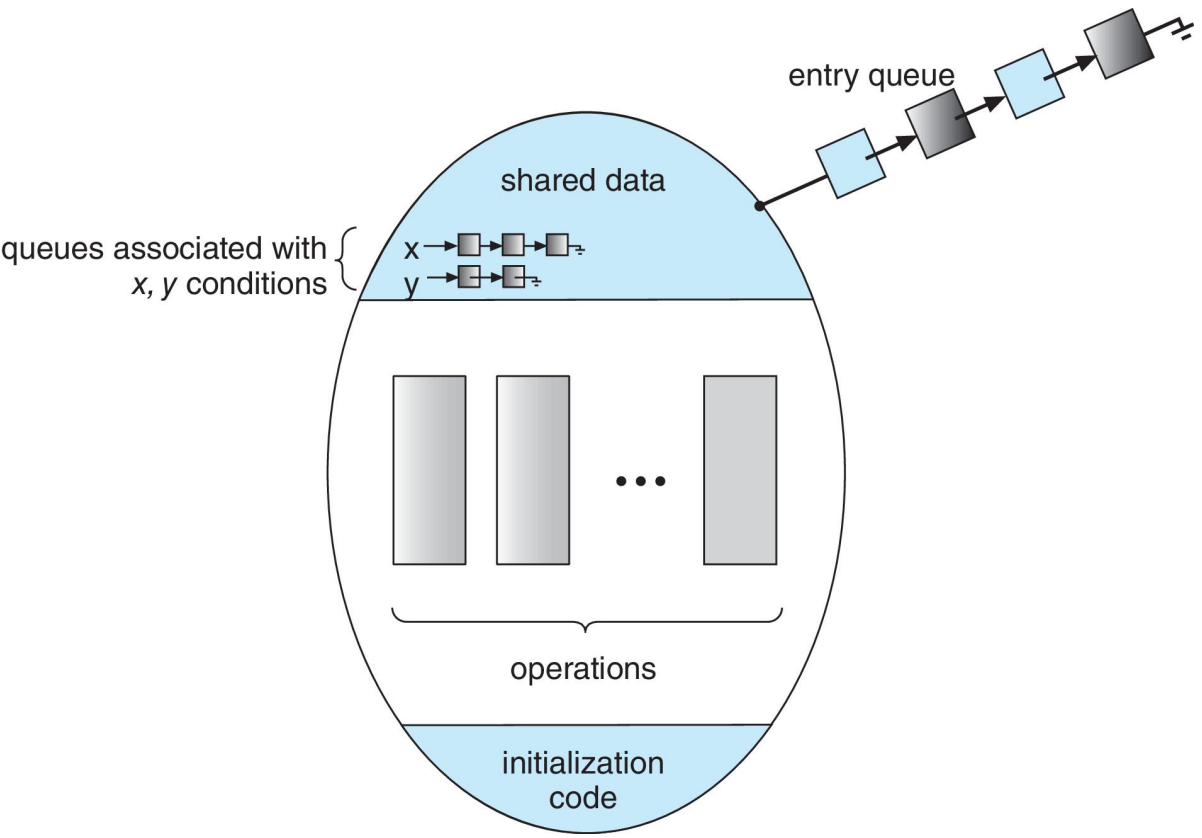
\includegraphics[width=0.6\linewidth]{img/condition_monitors.png}
    \caption{Monitor with Condition Variables}
\end{figure}

Usage of condition variable example:
\paragraph{}
Consider P1 and P2 that that need to execute two statements S1 and S2 and the requirement that S1 to happen before S2.

\begin{codeInC}
F1:
    S1;
    done = true;
    x.signal();
F2:
    if done = false
    x.wait()
    S2;
\end{codeInC}


\paragraph{Example: } variables 

\begin{itemize}
    \item[] semaphore mutex; // (initially = 1)
    \item[] semaphore next; // (initially = 0)
    \item[] int next\_count = 0; // number of processes waiting inside the monitor
\end{itemize}

Each function P will be replaced by

\begin{codeInC}
wait(mutex);
    ...
body of P;
    ...
if (next_count > 0)
    signal(next)
else
    signal(mutex);
\end{codeInC}

Mutual exclusion within a monitor is \textbf{ensured}.

\paragraph{}

For each condition variable x, we have:

\begin{itemize}
    \item semaphore x\_sem; // (initially = 0)
    \item int x\_count = 0;
\end{itemize}

\subsubsection{Implementation of x.wait() }

\begin{codeInC}
x_count++;
if (next_count > 0)
    signal(next);
else
    signal(mutex);
wait(x_sem);
x_count--;
\end{codeInC}

\subsubsection{Implementation of x.signal() }

\begin{codeInC}
if (x_count > 0) {
    next_count++;
    signal(x_sem);
    wait(next);
    next_count--;
}
\end{codeInC}

\subsection{Resuming Processes within a Monitor}
If several processes queued on condition variable x, and x.signal() is executed, which process should be resumed? \textbf{FCFS} may not be enough we can decide to pass a parameter inside the wait function.

\begin{itemize}
\centering
    \item[] \textbf{x.wait(c)}
\end{itemize}

where c is an integer (called the priority number). The process with lowest number (highest priority) is scheduled next. In this way the bounded waiting can be not respected. We can solve this be using ageing.

\newpage
\section{Single Resource allocation}
Allocate a single resource among competing processes using priority
numbers that specifies the maximum time a process plans to use the
resource.

The process with the shortest time is allocated the resource first

\paragraph{Example of access the resource}

\begin{codeInC}
R.acquire(t);
    ...
    access the resurce;
    ...
R.release;
\end{codeInC}

Where R is an instance of ResourceAllocator, and t is the maximum time a process plans to use the resource.


\begin{codeInC}
monitor ResourceAllocator{
    boolean busy;
    condition x;
    
    void acquire(int time) {
        if (busy)
            x.wait(time);
        busy = true;
    }
    void release() {
        busy = false;
        x.signal();
    }
    initialization code() {
        busy = false;
    }
}
\end{codeInC}

\newpage
\section{Liveness}
Processes may have to wait indefinitely while trying to acquire a synchronization tool such as a mutex lock or semaphore. Waiting indefinitely violates the progress and bounded-waiting criteria discussed at the beginning of this chapter.

\paragraph{}
Liveness refers to a set of properties that a system must satisfy to ensure processes make progress: \textbf{Indefinite waiting} is an example of a liveness failure because the bounded waiting is no satisfied.

\section{Deadlock}
Two or more processes are waiting indefinitely for an event that can be caused by only one of the waiting processes.

\paragraph{Example: } let S and Q be two semaphores initialized to 1.


\begin{figure}[htbp]
    \centering
    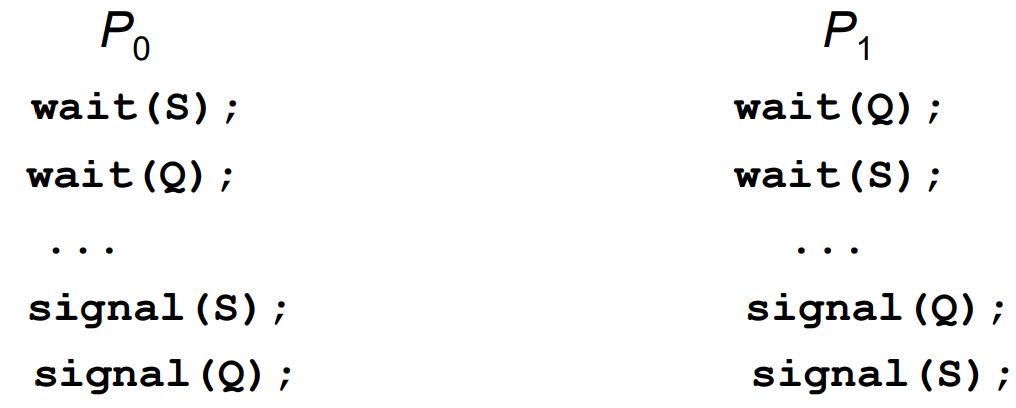
\includegraphics[width=0.5\linewidth]{img/witinskdijufb.png}
\end{figure}

Consider if P0 executes wait(S) and P1 wait(Q). When P0 executes
wait(Q), it must wait until P1 executes signal(Q)

However, P1 is waiting until P0 execute signal(S).

Since these signal() operations will never be executed, P0 and P1 are
deadlocked.

\subsection{Starvation}

Indefinite blocking. Process may never be removed from the semaphore queue in
which it is suspended

\subsection{Priority Inversion}

Scheduling problem when lower-priority process holds a lock needed by higher-priority process. This is solved via priority-inheritance protocol: when a task blocks one or more higher-priority tasks, it ignores its
original priority assignment and executes its critical section at the
highest priority level of all the tasks it blocks

\begin{figure}[htbp]
    \centering
    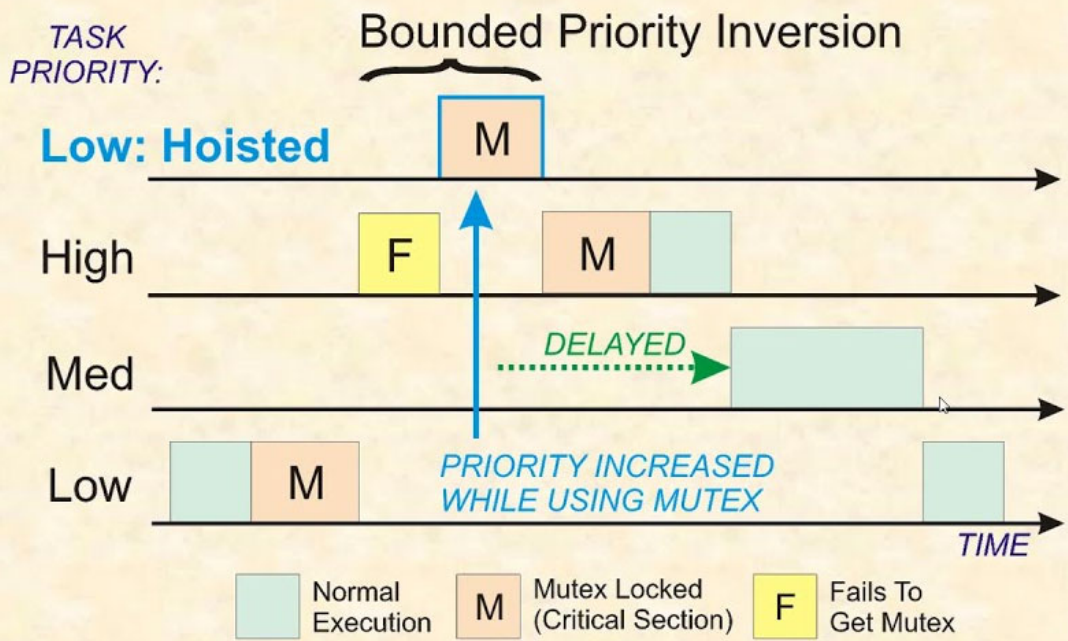
\includegraphics[width=0.5\linewidth]{img/adv.png}
\end{figure}

